We obtain the vertices of the rhombus as follows
\begin{align}
\vec{A} = \myvec{-3\\0},
\vec{B} = \myvec{0\\-3.5},
\vec{C} = \myvec{3\\0},
\vec{D} = \myvec{0\\3.5}
\end{align}
which are plotted in Fig. \ref{quad/45/fig:Rhombus ABCD}.
%
\begin{figure}[ht!]
\centering
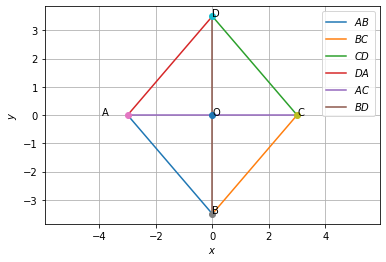
\includegraphics[width=\columnwidth]{solutions/quad/45/figure2.png}
\caption{Rhombus ABCD}
\label{quad/45/fig:Rhombus ABCD}
\end{figure}
